\section{Introduction}
%%%%%%%%%%%%%%%%%%%%%%%%%%%%%%%%%%%%%%%%%%%%%%%%%%%%%%%%%%%%%%%%%%%%%%%%
\begin{frame}
    \frametitle{SNe Classification}
    \begin{figure}[t]
        \centering
        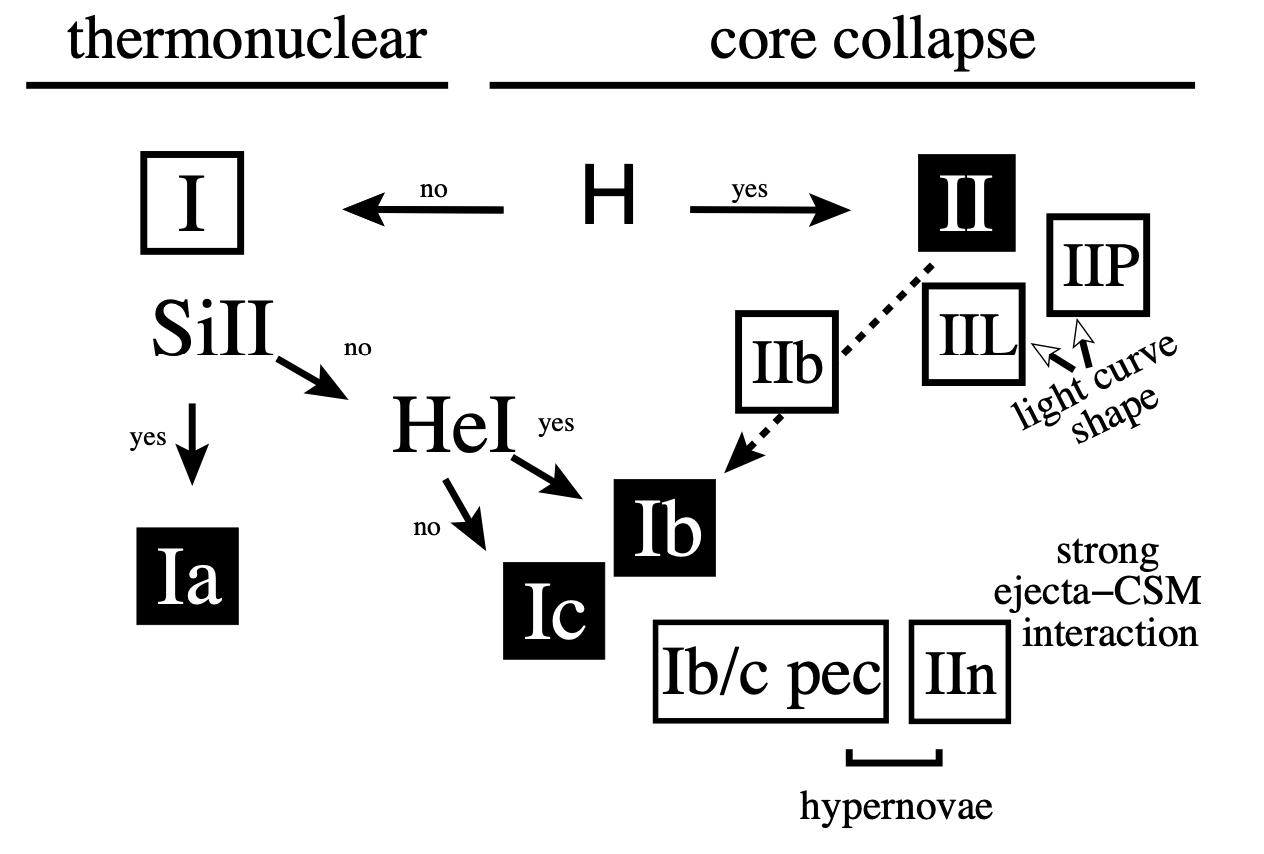
\includegraphics[width=0.7\linewidth]{figures/supernova_class.png }
        \caption{Supernova Classification Scheme (Adapted from  \textcite{Turatto2003}}
        % ]{Supernova classification. The 
        % classification scheme is based on the presence or absence of hydrogen and 
        % silicon features in the spectra of SNe. Figure from}
        \label{fig:sn-classification}
    \end{figure}
\end{frame}

\begin{frame}{DESI}
    \begin{itemize}
        \item Located at Kitt Peak National Observatory, Az
        \item Capable of resolving the [O II] $\lambda \lambda3726,3729$ doublet \parencite{Guy2023}
        \item Bright Galaxy Survey (BGS): $z<0.5$, $\sim10^5$ observed SNe! \parencite{desicollaboration2016, hahn2022}
    \end{itemize}
% The DESI survey focuses on four classes of targets: 14 million bright galaxies\footnote{The BGS contains galaxies with $r$-band magnitudes above 19.5.} in a Bright Galaxy Survey (BGS) at redshifts $z<0.5$; 8 million luminous red galaxies (LRGs) at redshifts $0.4<z<1.2$; 17 million emission line galaxies (ELGs) at $0.6<z<1.6$; and 3 million quasi-stellar objects (QSOs) between $0.9<z<4$. In this work, we will focus on the Bright Galaxy Survey, which is observing host galaxies with a median redshift of $z\approx0.2$ \parencite{desicollaboration2016, hahn2022}.
% DESI began its main survey in May 2021. Over the five-year span of observations, DESI will inevitably observe host galaxies with active SNe, leading to 
% contaminated spectra. The BGS may contain as many as $\sim10^5$ serendipitously observed supernova 
% \parencite{desicollaboration2016}. An example of a supernova observed in a BGS host by DESI and with an independent spectroscopic classification is shown in 
% The presence of transients in DESI spectra is a contaminant for the survey's dark energy program, since the transient can cause a catastrophic failure in the redshift fit, as shown in Figure~\ref{fig:desi_supernova_fail}. Thus it is useful to identify these contaminants whenever possible. Moreover, the serendipitous observation of supernovae is inherently useful since the spectroscopy provides an opportunity to classify {\sl most} types of supernovae without requiring additional follow-up. Both of these factors motivate this study.
\end{frame}

\begin{frame}{DESI Spectra SNe Classification}
    \begin{figure}[t]
        \centering
        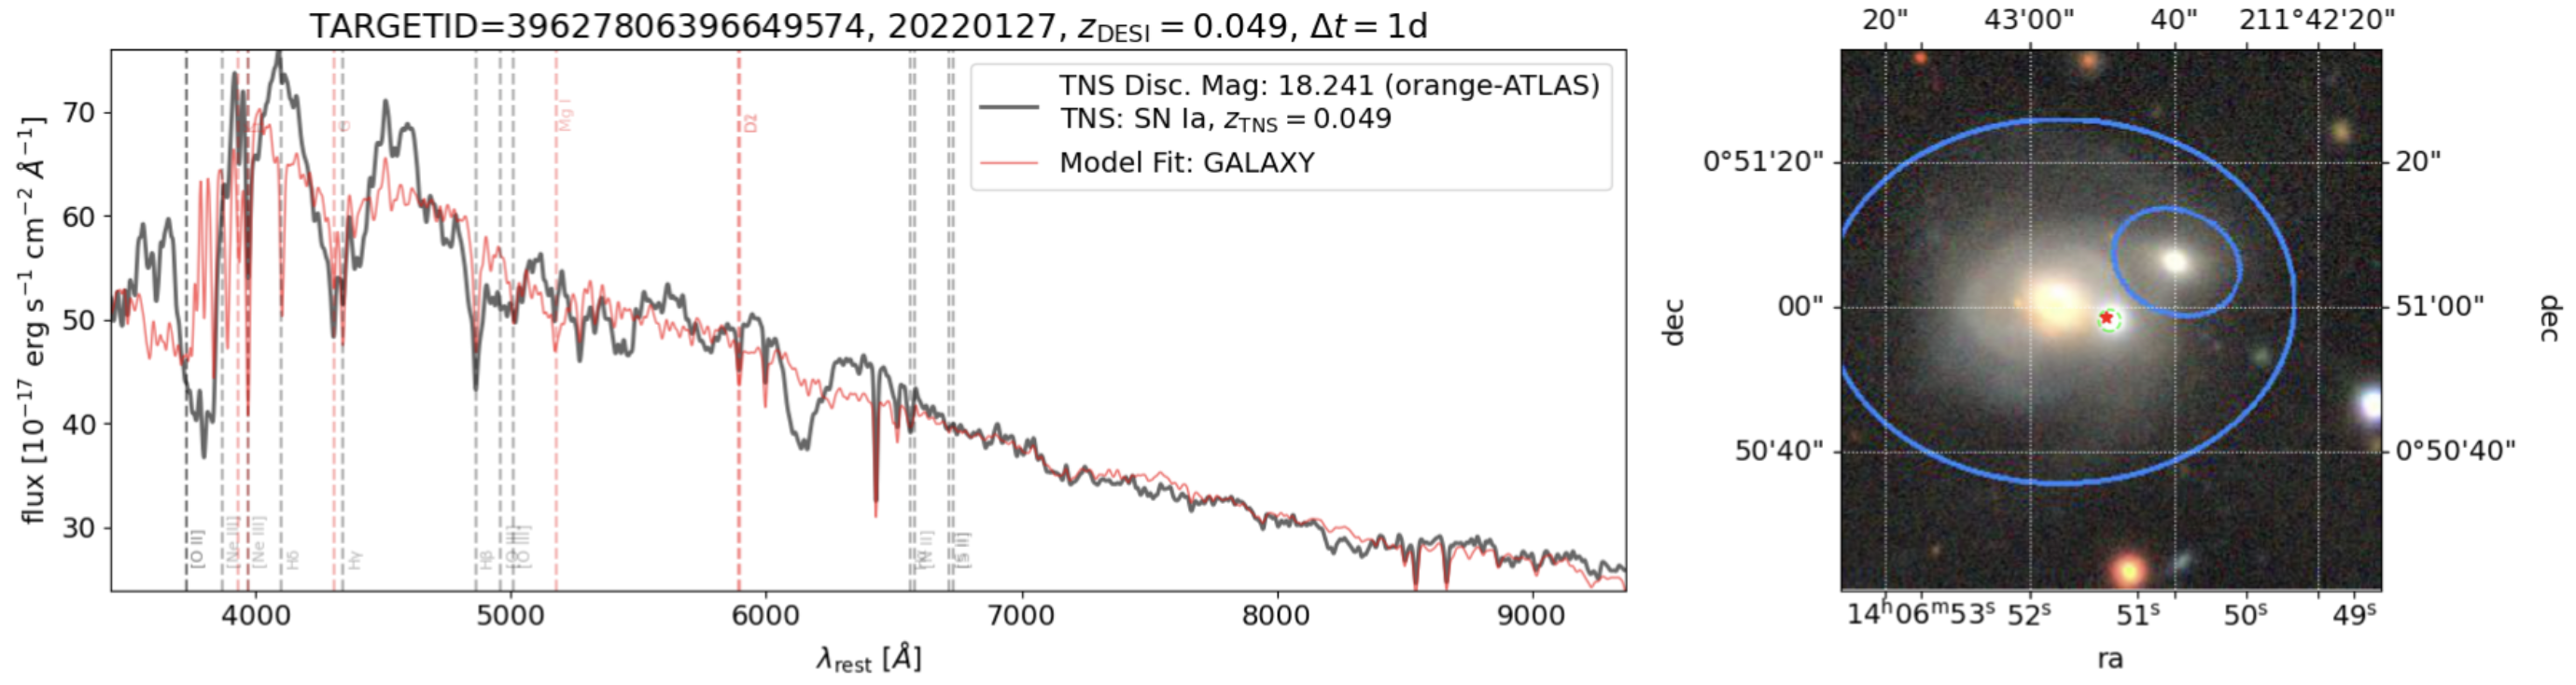
\includegraphics[width=\textwidth]{figures/desi_figures/SNe_Detection.png}
        \caption{DESI Spectra of Publicly Classified SNe Type Ia}
        % captured by DESI]{DESI host galaxy spectrum contaminated by a Type Ia supernova (January 2022). The right panel shows the image of the host galaxy, with the red star indicating the position of the DESI fiber. Independent spectroscopic follow-up reported to the TNS public database confirmed this is an SN Ia.}
        \label{fig:desi_supernova}
%     \end{figure}
% \end{frame}
% \begin{frame}
%     \begin{figure}[t!]
%         \centering
        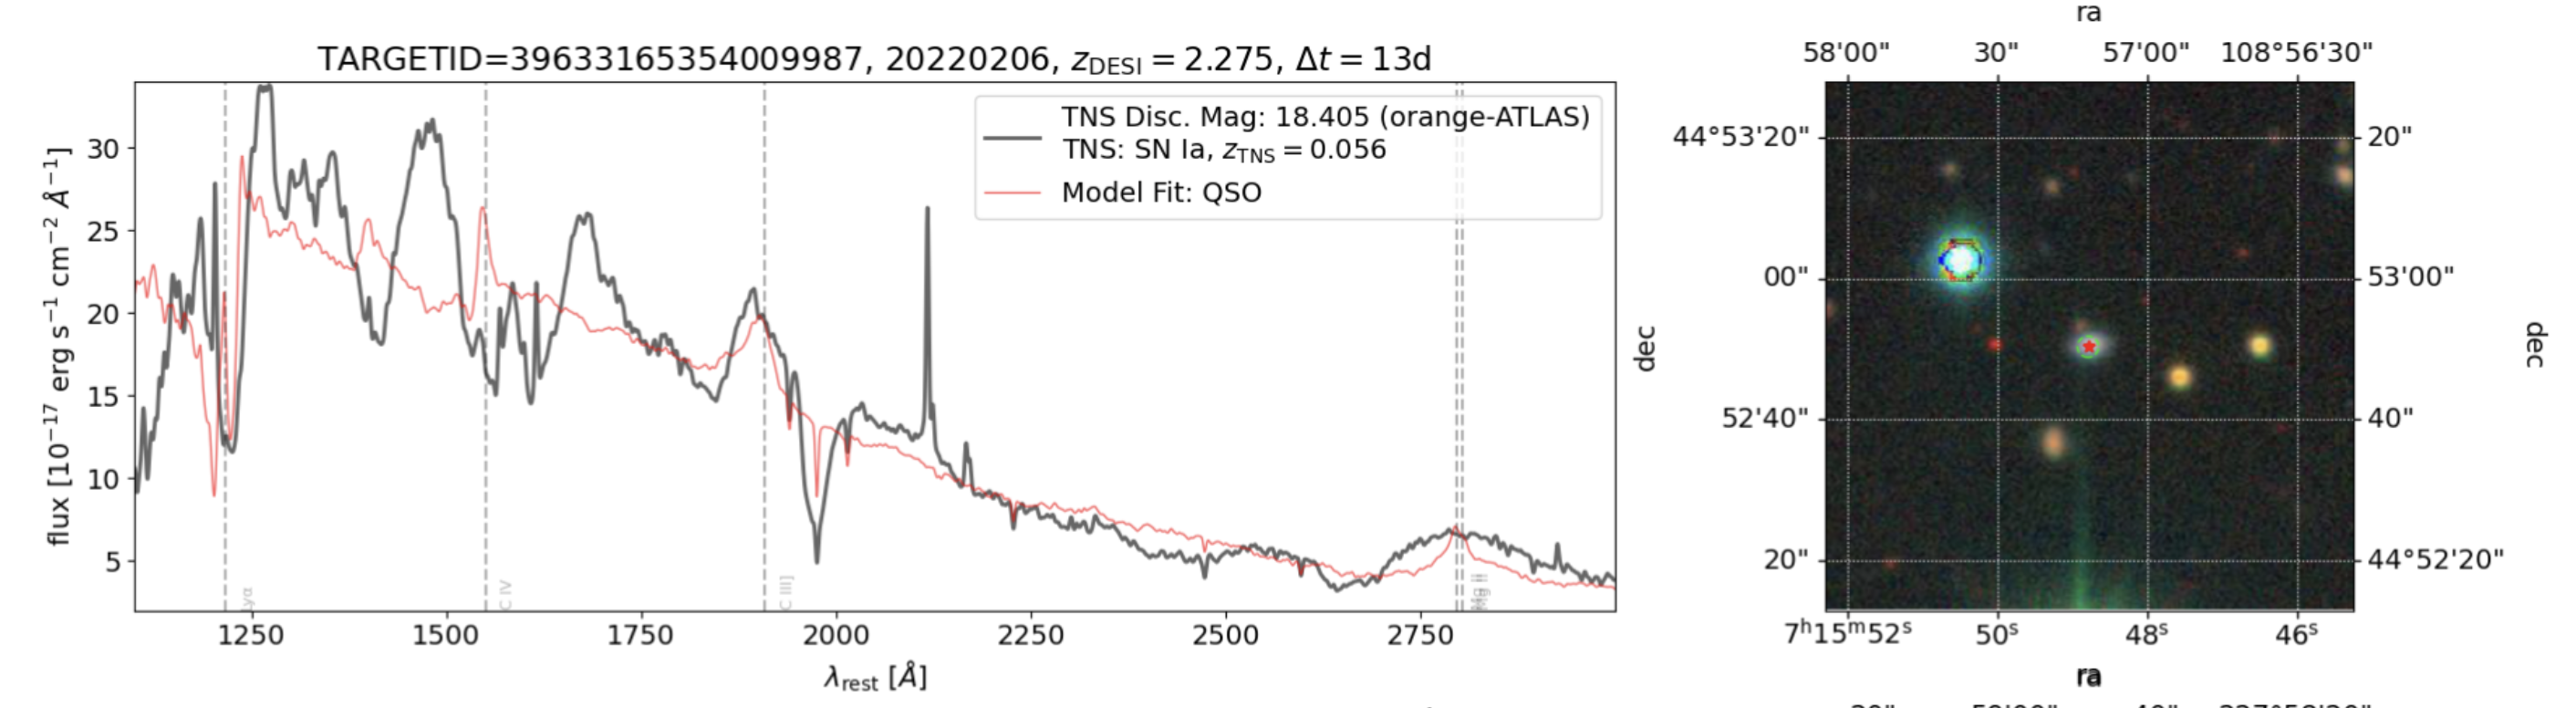
\includegraphics[width=\textwidth]{figures/desi_figures/SNe_detection_desifail.png}
        \caption{DESI Spectra of Publicly Classified SNe Type Ia -- Bad Redshift Fit}
        % Influencing DESI Redshift Fit]{DESI host galaxy spectrum contaminated by a Type Ia supernova (February 2022). The right panel shows the image of the host galaxy, with the red star indicating the position of the DESI fiber. Independent spectroscopic follow-up reported to the TNS public database confirmed this is an SN Ia. Note the extremely poor redshift fit provided by the DESI pipeline.}
        \label{fig:desi_supernova_fail}
    \end{figure}
\end{frame}


\begin{frame}{SNe Template}
    \begin{figure}[t]
        % \centering
        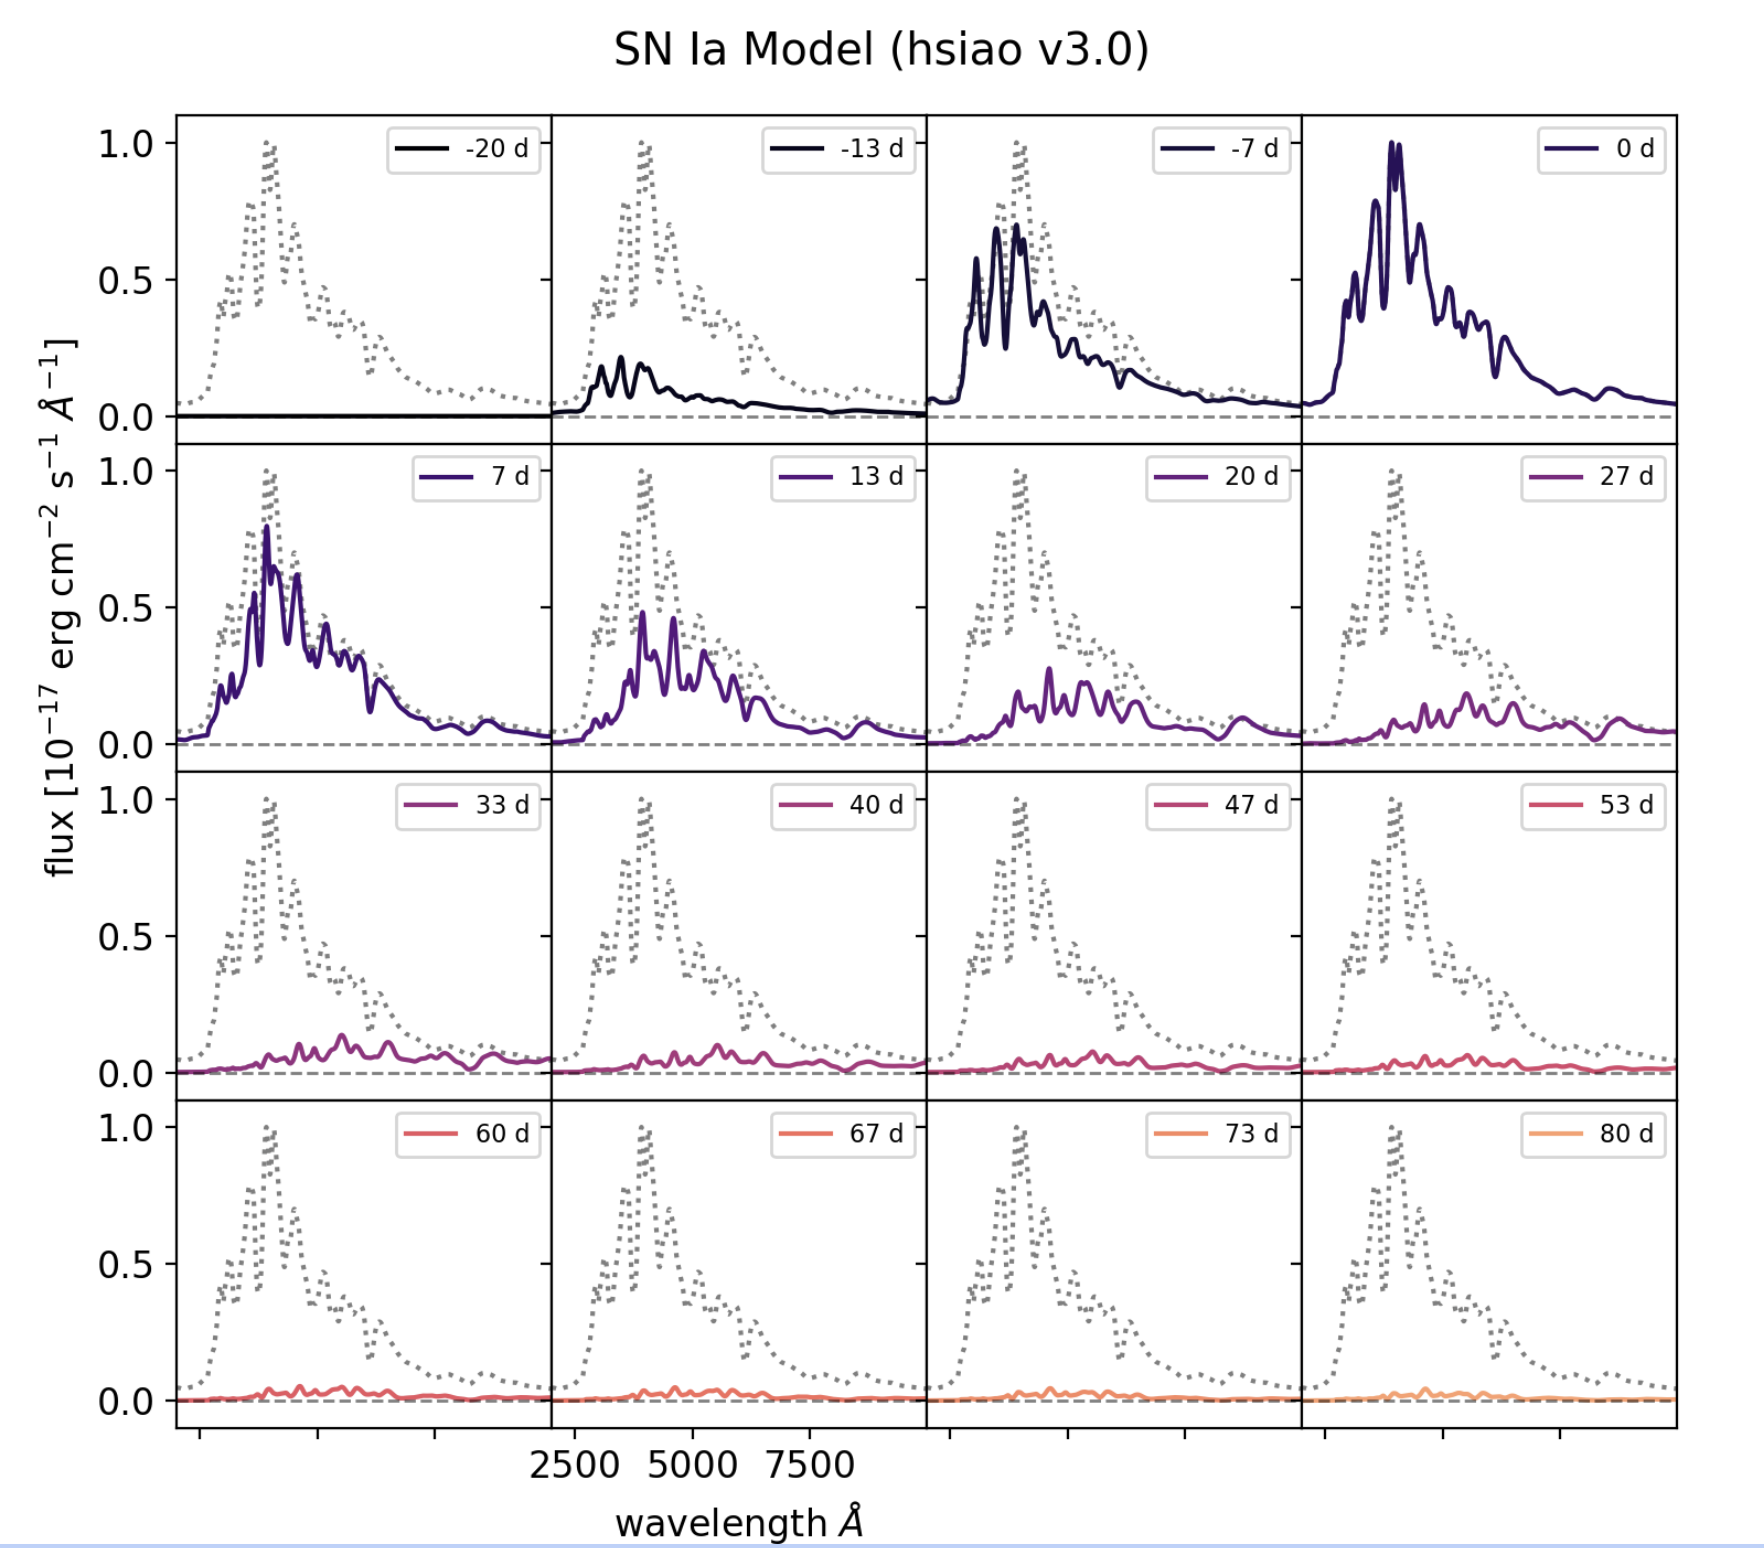
\includegraphics[width=.6\textwidth]{figures/desi_figures/snia_templates.png}
        \caption{Spectral Template of SN Ia SNe (-20$\to$ +80 days after peak) Adapted from \textcite{DESIpresentation}}
        % ]{Spectral model of a SN Ia shown over the course of its evolution, from 20 days before peak brightness to 80 days after. .}
        \label{fig:sne_template}
    \end{figure}
\end{frame}

\begin{frame}{DL in DESI Transient Analysis}
\begin{itemize}
    \item 1D CNN \parencite{wasserman2021}
    \item 2D CNN \parencite{Sepeku2022}
\end{itemize}
Problem: High precision, Low recall
\end{frame}


\begin{comment}
\begin{frame}
    \frametitle{Deep Learning in Medicine}
    \begin{itemize}
        \item<1-> Increase in demand for doctors time \cite{Zhang2020}
        \item<2-> Years of training required to interpret images, yet still inaccuracies occur 
        \item<3-> Helps identify rare diagnosis
    \end{itemize}
\end{frame}
\begin{frame}
    \begin{itemize}
        \item<1-> Small amount of legally available data (HIPAA) 
        \item<2-> Even smaller amount of labeled data (both for classification and segmentation tasks)
        \item<3-> Limited computational resources
        \item<4-> Fear of `black box' solutions
        \item<5-> Solution? Foundational models!
    \end{itemize}
\end{frame}
%%%%%%%%%%%%%%%%%%%%%%%%%%%%%%%%%%%%%%%%%%%%%%%%%%%%%%%%%%%%%%%%%%%%%%%%
\begin{frame}
    \frametitle{Foundational Models}
    \begin{columns}
    \column{0.5\textwidth}
    \begin{figure}
        \centering
        
\includegraphics[width=\linewidth]{figures/blackbox.jpeg}
        \caption{\cite{he2015ResNet}}
    \end{figure}
    \column{0.5\textwidth}
    \begin{figure}
        \centering
        
\includegraphics[width=\linewidth]{figures/blackbox.jpeg}
        \caption{\cite{Liu2021V2}}
    \end{figure}
    \end{columns}
        \begin{figure}
        \centering
        
\includegraphics[width=\linewidth]{figures/blackbox.jpeg}
        \caption{\cite{Long2014}}
    \end{figure}
\end{frame}
%%%%%%%%%%%%%%%%%%%%%%%%%%%%%%%%%%%%%%%%%%%%%%%%%%%%%%%%%%%%%%%%%%%%%%%%
\begin{frame}
    \frametitle{This Is anotherFrame}
    \resizebox{\linewidth}{!}{\begin{tikzpicture}[
    2d-arr/.style={matrix of nodes, row sep=-\pgflinewidth, column sep=-\pgflinewidth, nodes={draw}}
  ]

  \matrix (mtr) [2d-arr] {
  |[fill=red!30]| 0  & |[fill=red!30]| 0  & |[fill=red!30]| 0  & |[fill=red!30]| 0  & |[fill=red!30]| 0  & |[fill=red!30]| 0 \\
  |[fill=red!30]| 0  & |[fill=orange!30]| 1 & |[fill=orange!30]| 1 & |[fill=orange!30]| 1 &  0 & |[fill=red!30]| 0 \\
  |[fill=red!30]| 0  & |[fill=orange!30]| 0 & |[fill=orange!30]| 1 & |[fill=orange!30]| 1 &  1 & |[fill=red!30]| 0 \\
  |[fill=red!30]| 0  & |[fill=orange!30]| 0 & |[fill=orange!30]| 1 & |[fill=orange!30]| 1 & 0 & |[fill=red!30]| 0 \\
  |[fill=red!30]| 0  & 1 & 1 & 0 & 0 & |[fill=red!30]| 0 \\
  |[fill=red!30]| 0  & |[fill=red!30]| 0  & |[fill=red!30]| 0  & |[fill=red!30]| 0  & |[fill=red!30]| 0  & |[fill=red!30]| 0 \\
  };

  \node[below=of mtr-5-4] {$4\times4$ input with padding};

  \node[right=0.2em of mtr] (str) {$*$};

  \matrix (K) [2d-arr, right=0.2em of str, nodes={draw, fill=teal!30}] {
    1 & 0 &1\\
    0 & 1 &0\\
    1 & 0 & 1\\
  };
  \node[below=of K-2-2] {$3\times3$ filter};

  \node[right=0.2em of K] (eq) {$=$};

  \matrix (ret) [2d-arr, right=0.2em of eq] {
  2 & 2 & 3 &  1\\
  2 & |[fill=blue!80!black!30]| 4 & 3 & 3\\
  2 & 3 & |[fill=orange!30]| 4 & |[fill=orange!30]| 1 \\
  2 & 2 & |[fill=orange!30]| 1 & |[fill=orange!30]| 1 \\
  };
  \node[below=of ret-4-3] {$4\times4$ tensor};

  \node[right=0.2em of ret] (ra) {$\xrightarrow[]{\text{Max Pooling}}$};

\matrix (pool) [2d-arr, right=0.2em of ra] {
  4 & 3 \\
  3 & |[fill=blue!80!black!30]| 4 \\
  };
  \node[below=of pool-2-2] {$2\times2$ tensor};

  \draw[dashed, teal] (mtr-2-4.north east) -- (K-1-1.north west);
  \draw[dashed, teal] (mtr-4-4.south east) -- (K-3-1.south west);

  \draw[dashed, blue!80!green] (K-1-3.north east) -- (ret-2-2.north west);
  \draw[dashed, blue!80!black] (K-3-3.south east) -- (ret-2-2.south west);

  \draw[dashed, blue!80!green] (K-1-3.north east) -- (ret-2-2.north west);
  \draw[dashed, blue!80!black] (K-3-3.south east) -- (ret-2-2.south west);

\draw[dashed, blue!80!green] (ret-3-4.north east) -- (pool-2-2.north west);
  \draw[dashed, blue!80!black] (ret-4-4.south east) -- (pool-2-2.south west);

\end{tikzpicture}
}
\end{frame}
%%%%%%%%%%%%%%%%%%%%%%%%%%%%%%%%%%%%%%%%%%%%%%%%%%%%%%%%%%%%%%%%%%%%%%%%
\begin{frame}
    \frametitle{ThisIsaFrame}
    \resizebox{\linewidth}{!}{\begin{tikzpicture}[x=2.2cm,y=1.4cm]
  \message{^^JNeural network without text}
  \readlist\Nnod{4,5,5,5,3} % array of number of nodes per layer
  
  \message{^^J  Layer}
  \foreachitem \N \in \Nnod{ % loop over layers
    \def\lay{\Ncnt} % alias of index of current layer
    \pgfmathsetmacro\prev{int(\Ncnt-1)} % number of previous layer
    \message{\lay,}
    \foreach \i [evaluate={\y=\N/2-\i; \x=\lay; \n=\nstyle;}] in {1,...,\N}{ % loop over nodes
      
      % NODES
      \node[node \n] (N\lay-\i) at (\x,\y) {};
      
      % CONNECTIONS
      \ifnum\lay>1 % connect to previous layer
        \foreach \j in {1,...,\Nnod[\prev]}{ % loop over nodes in previous layer
          \draw[connect,white,line width=1.2] (N\prev-\j) -- (N\lay-\i);
          \draw[connect] (N\prev-\j) -- (N\lay-\i);
          %\draw[connect] (N\prev-\j.0) -- (N\lay-\i.180); % connect to left
        }
      \fi % else: nothing to connect first layer
      
    }
  }
  
  % LABELS
  \node[above=5,align=center,mygreen!60!black] at (N1-1.90) {input\\[-0.2em]layer};
  \node[above=2,align=center,myblue!60!black] at (N3-1.90) {hidden layer};
  \node[above=10,align=center,myred!60!black] at (N\Nnodlen-1.90) {output\\[-0.2em]layer};
  
\end{tikzpicture}
}
\end{frame}
\end{comment}